%++++++++++++++++++++++++++++++++++++++++
% Don't modify this section unless you know what you're doing!
\documentclass[letterpaper,12pt]{article}
\usepackage{tabularx} % extra features for tabular environment
\usepackage{amsmath}  % improve math presentation
\usepackage{amssymb}
\usepackage{multirow}
\usepackage{graphicx} % takes care of graphic including machinery
\usepackage{pgfplots}
\pgfplotsset{width=10cm,compat=1.9}
\usepackage[margin=1in,letterpaper]{geometry} % decreases margins
\usepackage{cite} % takes care of citations
\usepackage[final]{hyperref} % adds hyper links inside the generated pdf file
\usepackage{tikz}
\usepackage{xcolor}
\usepackage{listings}
\usepackage{url}
\usepackage{tikz}
\usepackage{tzplot}
\renewcommand{\vec}[1]{\boldsymbol{#1}}
\hypersetup{
	colorlinks=true,       % false: boxed links; true: colored links
	linkcolor=blue,        % color of internal links
	citecolor=blue,        % color of links to bibliography
	filecolor=magenta,     % color of file links
	urlcolor=blue         
}
%++++++++++++++++++++++++++++++++++++++++

\title{PRML-Assignment 2}
\author{Rohith Ingilela,  EE19BTECH11005 }
\date{April 8, 2023}

\begin{document}

\maketitle

\section{Problem Statement}

In Figure \ref*{fig:fig1}, $ABCD$ is a parallelogram, $AE \perp DC$
and $CF \perp AD$. If $AB = 16 \hspace{0.1cm} cm$, $AE = 8 \hspace{0.1cm} cm$ and
$CF = 10 \hspace{0.1cm} cm$, find $AD$. Construct the paralellogram.

\begin{figure}[!ht]
\centering

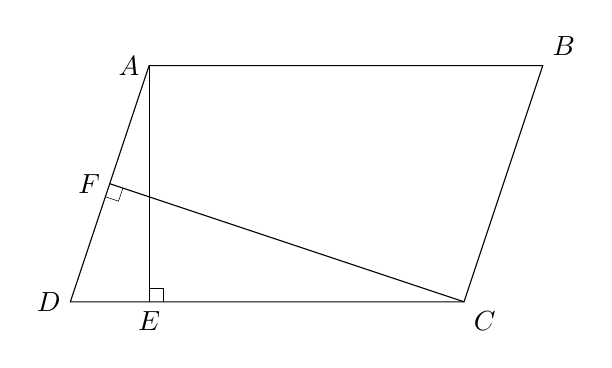
\begin{tikzpicture}
% triangle
\tzcoors(0,0)(D){$D$}[180](5,0)(C){$C$}[-45](6,3)(B){$B$}[45](1,3)(A){$A$}[180](1,0)(E){$E$}[-90](0.5,1.5)(F){$F$}[180];
\tzpolygon(A){}(B){}(C){}(D){};
\tzpolygon(A){}(E){};
\tzpolygon(C){}(F){};
% angle marks
\tzrightanglemark(D)(F)(C){}
\tzrightanglemark(A)(E)(C){}
\end{tikzpicture}

\caption{Parallelogram ABCD}
\label{fig:fig1}
\end{figure}
\section{Solution}

Given,

\setlength{\arrayrulewidth}{0.5mm}
\setlength{\tabcolsep}{30pt}
\setlength\extrarowheight{10pt}

\begin{center}
\begin{tabular}{||c|c||} 
 \hline
 \hline
 \textbf{LHS} & \textbf{RHS} \\
 \hline
 $\Vec{A}-\Vec{B}$ & $\Vec{C}-\Vec{D}$ \\
 \hline
 $(\Vec{A} - \Vec{E})^T (\Vec{C} - \Vec{D})$ & 0 \\
 \hline
 $(\Vec{C} - \Vec{F})^T (\Vec{A} - \Vec{D})$ & 0 \\
 \hline
 $\|\Vec{A} - \Vec{B}\|$ & 16 cm \\
 \hline
  $\|\Vec{A} - \Vec{E}\|$ & 8 cm \\
 \hline
 $\|\Vec{C} - \Vec{F}\|$ & 10 cm \\
 \hline
 \hline
\end{tabular}
\end{center}

\clearpage

To find: $\|AD\|$ \\

We know that,
\begin{center}
    $Ar(ABCD) = \|\Vec{A}-\Vec{D}\|\times\|\Vec{C}-\Vec{F}\| = \|\Vec{A}-\Vec{E}\|\times\|\Vec{C}-\Vec{D}\|$ \\
\end{center}
\begin{center}
    $\|\Vec{A}-\Vec{D}\| \times 10 = 8 \times 16 = 128$
\end{center}
\begin{center}
    $\|\Vec{A}-\Vec{D}\| = 12.8 \text{ } cm$
\end{center}
\begin{equation}
\nonumber
    \|\Vec{A} - \Vec{D}\| = \|\Vec{A}\| = 12.8 \text{ } cm
\end{equation}

To find: $\Vec{A}$ \\

Let $\theta = \angle ADE$
\begin{center}
    $\sin \theta = \frac{\|\Vec{A}-\Vec{E}\|}{\|\Vec{A}-\Vec{D}\|}$
\end{center}
\begin{equation}
    \theta = \sin^{-1}\left(\frac{\|\Vec{A}-\Vec{E}\|}{\|\Vec{A}-\Vec{D}\|}\right)
\label{eqntheta}
\end{equation}
\begin{equation}
    \Vec{A} = \|\Vec{A}-\Vec{D}\|\begin{pmatrix} \cos \theta \\ \sin \theta \end{pmatrix}
\label{eqnA}
\end{equation}
Substituting $\|AE\|$ and $\|AD\|$ in (\ref*{eqntheta}) and (\ref*{eqnA})
\begin{equation}
    \Vec{A} \approx \begin{pmatrix} 10 \\ 8 \end{pmatrix}
\end{equation}
To find: $\Vec{F}$ \\ \\
Equation of line passing through AD:
\begin{center}
    Direction vector, $\Vec{m} = \begin{pmatrix} 10 \\ 8 \end{pmatrix}$
\end{center}
Normal vector,
\begin{center}
    $\implies \Vec{n} = \begin{pmatrix} -8 \\ 10 \end{pmatrix}$
\end{center}
Equation of line passing through D with normal vector n is
\begin{center}
    $\Vec{n}^T(\Vec{x} - \Vec{D}) = 0$
\end{center}
\begin{equation}
    \Vec{n}^T\Vec{x} = 0
\end{equation}
Since $\Vec{F}$ is foot of perpendicular from $\Vec{C}$ to line $\Vec{AD}$
\begin{center}
    $\begin{pmatrix}m & n\end{pmatrix}^T\Vec{F} = \begin{pmatrix} m^TC \\ 0 \end{pmatrix}$
\end{center}
\begin{center}
    $\Vec{F} = \begin{pmatrix}10 & 8 \\ 8 & -10 \end{pmatrix}^{-1}\begin{pmatrix} 160 \\ 0 \end{pmatrix}$
\end{center}
\begin{equation}
    \Vec{F} = \begin{pmatrix}9.75 \\ 7.8\end{pmatrix}
\end{equation}

\clearpage

\section{Code}
\url{https://github.com/1R0H1TH/PRML/blob/main/9.9.2.1/codes/9.9.2.1.py}

\section{Plot}
The above code plots Figure \ref{fig:fig2}.
\begin{figure}[!ht]
\centering
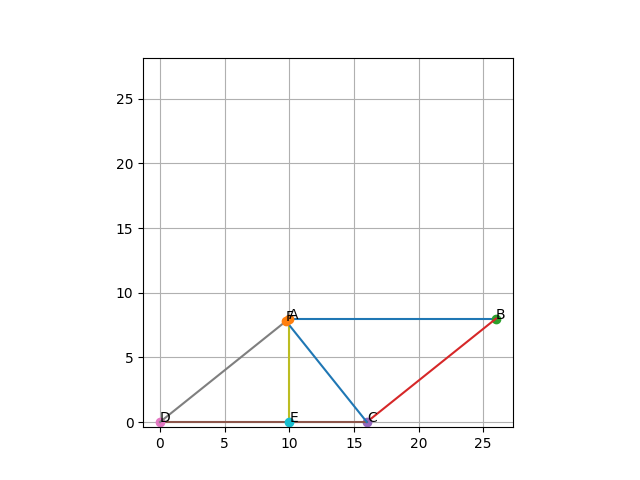
\includegraphics[width=0.75\columnwidth]{figs/Figure_1.png}
\caption{Parallelogram ABCD}
\label{fig:fig2}
\end{figure}.


\end{document}
